\documentclass{beamer}
\usetheme{Dresden}
\usecolortheme{beaver}
\usepackage{algpseudocode}
\usepackage{listings}
\usepackage{xcolor}
\usepackage[outdir=./]{epstopdf}
\lstset{
	language=C++,
	backgroundcolor=\color{black!5}, % set backgroundcolor
	basicstyle=\footnotesize\ttfamily,% basic font setting
	columns=fullflexible,
}

\begin{document}

\title{Q-Learning Parallelization}
\author{Jacopo Di Simone}
\institute{Politecnico di Milano, Milano, Italia}
\date{5 May, 2017}
\beamertemplatenavigationsymbolsempty

\begin{frame}
\titlepage
\end{frame}

\begin{frame}{Introduction}
\begin{itemize}
\item The goal of the project was to parallelize the Reinforcement Learning algorithm Q-Learning, used for solving tasks modeled after Markov Decision Processes (learn the optimal policy). The technique is described in the paper "A parallel implementation of Q-Learning based on communication with cache" of Printista et al.
\item The idea of the algorithm is to let an agent act in an environment, collect its reward and update the q-function.
\item The main characteristics of Q-Learning method is the ability to learn the optimal q-function (and the optimal policy) following a non optimal policy.
\end{itemize}
\end{frame}

\begin{frame}{Sequential Q-Learning}
\begin{algorithmic}
\State Initialize $Q(s,a) \  \forall s \in S$ and $\forall a \in A(s)$
\ForAll{episodes}
	\State Initialize $s$
	\Repeat
   		\State Choose $a$ from $s$ using a $\epsilon$-greedy policy derived from Q
   		\State Take action $a$, observe resultant state $s'$ and the reward $r$
   		\State $Q(s,a) \leftarrow Q(s,a) + \alpha + [ r + \gamma \max Q(s',a') - Q(s,a )]$
	\Until{$s$ is terminal}
\EndFor
\end{algorithmic}
\end{frame}

\begin{frame}{Parallel Q-Learning}
\begin{itemize}
\item In the paper the author propose a parallelization of the algorithm of the type Domain Data Decomposition.
	\begin{itemize}
	\item The data are decomposed in different chunk. In our case the data is the q-function.
	\item Each task will work on a chunk.
	\end{itemize}
\end{itemize}
\end{frame}

\begin{frame}{Proposed Implementation: Process}
In the algorithm there are 2 type of tasks: \emph{Slave} and \emph{Master}.
\begin{itemize}
\item The tasks \emph{Slave} will handle the computational part, applying the Q-Learning method to the assigned domain.
\item The task \emph{Master} will handle the communication in the program and will conserve a global version of the q-function.
\end{itemize}
\end{frame}

\begin{frame}{Proposed Implementation: Communication}
The communication are always between Slave and Master and never between Slave and Slave.
\begin{itemize}
\item \emph{reqmsg} is sent from task \emph{Slave} to ask for value of the q-function out of its domain. To avoid high communication overhead it was implemented a cache. It keeps the last value provided by the master until a certain requirement is reach. After that a new \emph{reqmsg} is sent.
\item \emph{infmsg} is periodically sent from the \emph{Slave} to the \emph{Master} with their q-function partition. Also in this case to avoid the overhead the message is sent every \emph{tot} epoch.
\end{itemize}
\end{frame}

\begin{frame}{Implementation: Idea}
\begin{itemize}
\item The algorithm is implemented in C++ using the pthread library.
\item Unlike the implementation proposed in the paper, the \emph{Master} was eliminated. In its place the concept of shared memory was adopted: a memory shared between every tasks.
\end{itemize}
\end{frame}

\begin{frame}[fragile]{Implementation: Q-Learning}
The Q-Learning function is implemented in the Agent class through the function \emph{learn}
\begin{lstlisting}
/*
static function used to run the q learning function by an agent
@param agent: agent which learn the function. Passed as a pointer
of void just to satisfy some constraints of pthread
*/
static void * learn(void * agent);
\end{lstlisting}
\end{frame}

\begin{frame}{Implementation: Problem}
\begin{columns}
	\begin{column}{0.5\textwidth}
	 To test the algorithm I selected the same problem used in the paper; the grid. Each transition in the grid give a reward of $0$, except for the 2 goal state which give a reward of 100. The game terminate when the agent reach a goal. The disocunt factor is $\gamma$ is $0.95$.
	\end{column}
	\begin{column}{0.5\textwidth}  %%<--- here
		\begin{center}
			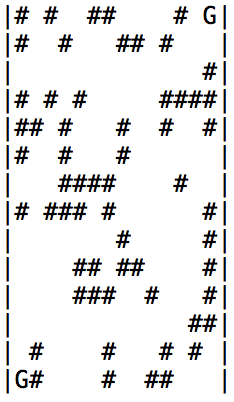
\includegraphics[width=0.5\textwidth]{grid.png}
		\end{center}
	\end{column}
\end{columns}
\end{frame}

\begin{frame}[fragile]{Implementation: Environment}
To handle the interaction of the Agent in the grid I created the class Environment. Through many functions allow the agent to act in the grid. One of this functions is \emph{step}.
\begin{lstlisting}
/*
make a step in the grid (modify also the curr_state variable)
@param action to be performed
@return the observation: next_state (integer (-1 if the 
			    state is goal)), reward, done
*/
observation step(Actions a);
\end{lstlisting}
\end{frame}

\begin{frame}[fragile]{Implementation: Optimal Value Function}
To test the algorithm and obtain the optimal Value function I used the Value Iteration method. This is implemented in the Environment class through the function \emph{valueiteration}.
\begin{lstlisting}
/*
@param env: environment to learn
discount factor
theta: precision of the algorithm (default 0)
@return value function as a (pointer to) vector of double
*/
std::shared_ptr<Eigen::VectorXd> valueIteration(
                                      double discount_factor = 0.95,
                                      double theta = 0);
\end{lstlisting}
\end{frame}

\begin{frame}{Results analysis: Execution Times}
   The results are obtained doing a mean over 30 execution for each number of tasks (1, 2, 4). Then I collect these measurements with the ones of 10 other different grids, doing a mean of the obtained results.
\begin{table}
\centering
\begin{tabular}{| l | l | l | l |}
\hline
\emph{np} & 1 & 2 & 4\\
\hline
Tempo & 3.8167 & 2.8311 & 1.9521\\
\hline
Speedup & -------- & 1.346 & 1.783\\
\hline
\end{tabular}
\end{table}
\end{frame}

\begin{frame}{Results analysis: Learning rate}
In the graph are represented the learning rate curves for 4 different number of processes (1,2,4,8). These are computed doing a percentage of the learned states in each episode and computing the mean over all 11 grids.
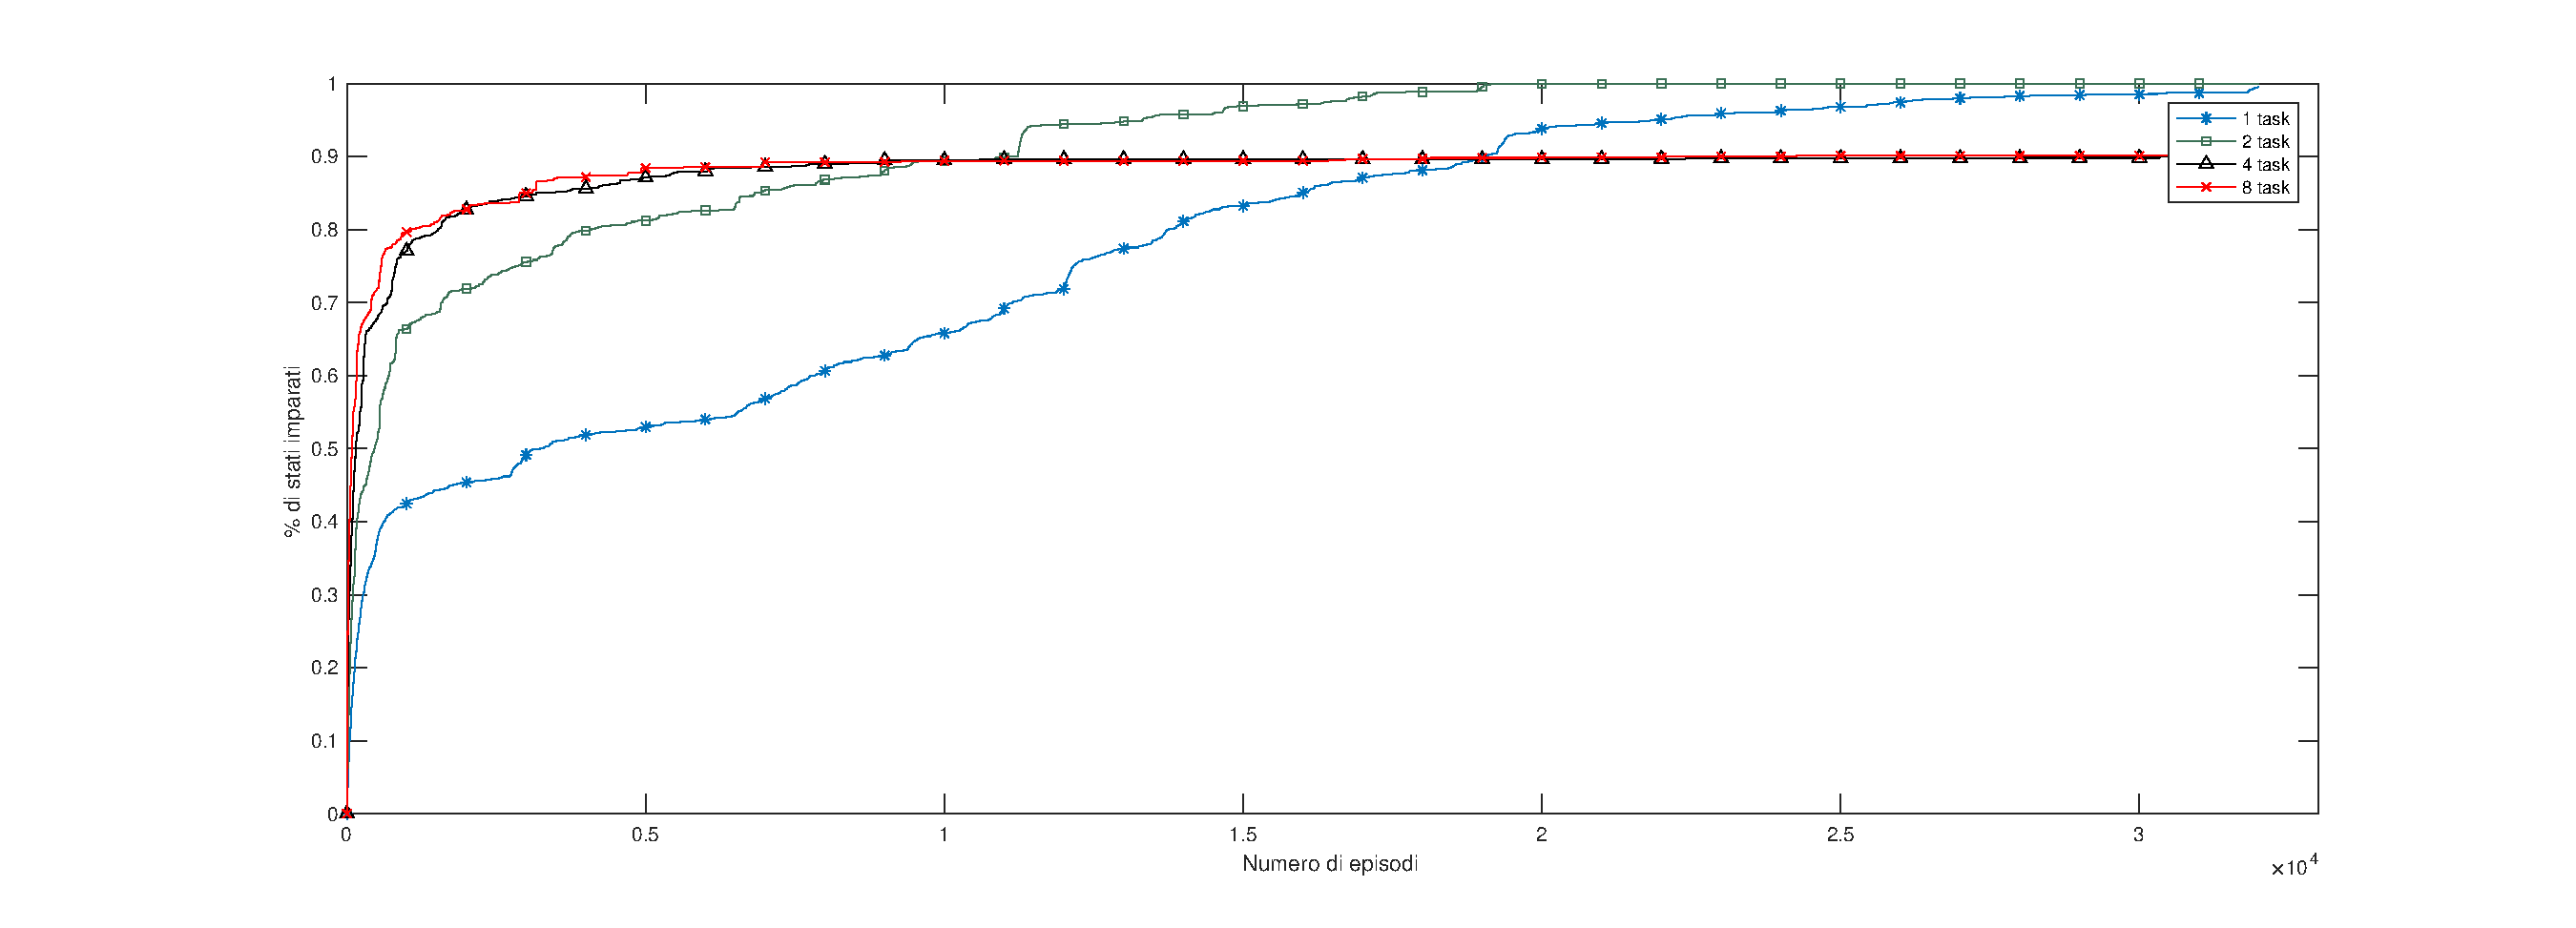
\includegraphics[height=4cm]{per_learned_states}
\end{frame}

\begin{frame}{Conclusions}
The obtained results regarding the execution time are what I expect, according also to the results showed in the paper.
~\\~\\
Instead, the learning rate did not give the expected results. This is due to the $\epsilon$ value used in the experiment ($0.1$). Being this value so low, it give to much credit to the initial explored state, assigning a probability too low to action without the maximum expected value. Using an $\epsilon$ that change its value episode per episode remove this problem.
\end{frame}

\end{document}